\chapter{Betriebsmittel}
\label{betriebsmittel}
Als Betriebsmittel werden hier auszuleihende Gegenst�nde wie Zutrittskarten oder Schl�ssel verstanden.
\section{Aufbau der Karteikarte Betriebsmittel}
Die Abbildung \ref{Betriebsmittel1} zeigt den Aufbau der Karteikarte \textsl{Betriebsmittel}:
\begin{itemize}
	\item Listenfeld: Hier werden alle Betriebsmittel, die der Student ausgeliehen hat angezeigt.
	\item Details-Bereich: Im Details-bereich k�nnen die Betriebsmitteldaten eingegeben und ver�ndert werden.
	\begin{itemize}
		\item Typ: Welcher Gegenstand wurde entliehen. Auswahl z.Z.: Schl�ssel, Zutrittskarte, Laptop.
		\item Nummer: Schl�sselnummer bzw Kartennummer
		\item Nummer 2: Feld f�r die zweite Kartennummer (zb bei Dualtranspondern)
		\item Inventarnummer: Feld zur Auswahl der Inventarnummer
		\item Beschreibung: Zus�tzliche Informationen zum Betriebsmittel.
		\item Kaution: Einbezahlte Kaution.
		\item Anmerkung: Zus�tzliche Informationen zur Entleihung.
		\item Ausgegeben am: Datum der Ausgabe.
		\item Retour am: Datum der R�ckgabe.
	\end{itemize}
	\item Button \textsl{Neu}: Start der Eingabe einer Betriebsmittelentlehnung.
	\item Button \textsl{Loeschen}: L�schen eines markierten, fehlerhaften Eintrags.
	\item Button \textsl{�bernahmebest�tigung}: Hier wird eine �bernahmebest�tigung f�r das gew�hlte Betriebsmittel erstellt
\end{itemize}
\begin{figure}
	\centering
	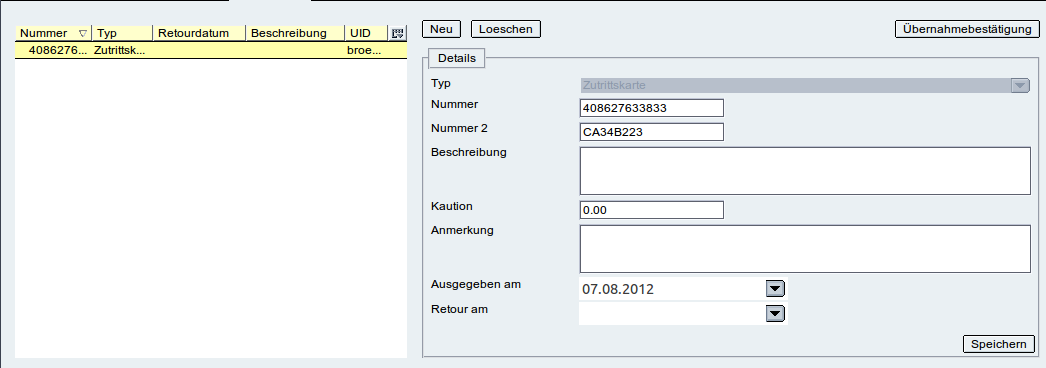
\includegraphics[width=0.75\textwidth]{FAS_Betriebsmittel1.png}
	\caption{Die Karteikarte Betriebsmittel}
	\label{Betriebsmittel1}
\end{figure}
\section{Eingabe von Betriebsmittelentlehnungen}
\underline{Beispiel}:\\
Student XY erh�lt einen Laptop vom Studiengang f�r seine Projektarbeit.
Nach der Auswahl des Studenten wird die Karteikarte \textsl{Betriebsmittel} ge�ffnet und mit der Taste \textit{Neu} der Eingabevorgang begonnen. Zuerst wird bei Typ \textsl{Inventar} ausgew�hlt. Nun wird statt den Nummern-Feldern ein Inventarnummer Feld angezeigt. Hier wird die Inventarnummer des Laptops eingetragen (zB 88+02+0005). Hier kann auch nur ein Teil der Inventarnummer eingetragen werden, die gefundenen Vorschl�ge werden nach dem Eintippen im Dropdown angezeigt. Zuletzt wird noch das aktuelle Datum als Entlehndatum eingegeben. Abgeschlossen wird der Eingabevorgang durch Klicken der Taste \textsl{Speichern}.\\
Damit das Inventar hier gefunden wird, muss dieses zuerst inventarisiert werden. Dies geschieht im Vilesci unter \textsl{Inventar}\\
\underline{Beispiel}:\\
Student XY erh�lt zum Studienbeginn die Zutrittskarte mit der Nummer 408627633833. \\
Nach der Auswahl des Studenten wird die Karteikarte \textsl{Betriebsmittel} ge�ffnet und mit der Taste \textit{Neu} der Eingabevorgang begonnen. Zuerst wird bei Typ \textsl{Zutrittskarte} ausgew�hlt, dann darunter die Nummer 408627633833 der Zutrittskarte in das linke Feld eingegeben. Im Feld \textsl{Beschreibung} k�nnte jetzt noch eine genauere Beschreibung der Zutrittskarte eingegeben werden. Dann wird der Betrag der Kaution eingegeben. Zuletzt wird noch das aktuelle Datum als Entlehndatum eingegeben. Abgeschlossen wird der Eingabevorgang durch Klicken der Taste \textsl{Speichern}.\\
\underline{Beispiel}:\\
Student XY hat sein Studium beendet und will seine Zutrittskarte zur�ckgeben.\\
Nach der Auswahl des Studenten wird der Karteikarte \textsl{Betriebsmittel} ge�ffnet und die Eintragung mit der Nummer der Zutrittskarte im Listenfeld markiert. Jetzt kann das R�ckgabedatum in das Feld \textsl{Retour am} eingetragen werden. Durch Klicken der Taste \textsl{Speichern} wird der Datensatz aktualisiert und das R�ckgabedatum gespeichert.\\
\underline{Beispiel}:\\
Student YZ ist seine Zutrittskarte leider abhanden gekommen.\\
In diesem Fall wird im \textsl{Anmerkung}-Feld vermerkt, da� der Student YZ am heutigen Tag den Verlust der Karte gemeldet hat und das \textsl{Retour am}-Feld auf das aktuelle Datum gesetzt.